\chapter{Additional plots}
\label{ch:additional_plots}
This appendix contains extra plots that may be useful, but were not included in the main document.
\clearpage

\section{Quasi-stativ \acs*{vs} fall simulator subfailure}
\label{sec:additional_QS_FS}

\begin{figure}[h]
\centering
\includegraphics[width=\linewidth]{./appendixPlots/figures/StrainVsStrain}
\caption[Quasi-static vs.\ fall simulator strain]{\textbf{Minimum principal strain at the location of the strain gauge in the fall simulator and in the quasi-static testing at the maximum force applied in the quasi-static test.} Graphic \copyright Seth Gilchrist, 2013.}
\label{fig:StrainVsStrain}
\end{figure}
\clearpage

\begin{figure}[h]
\centering
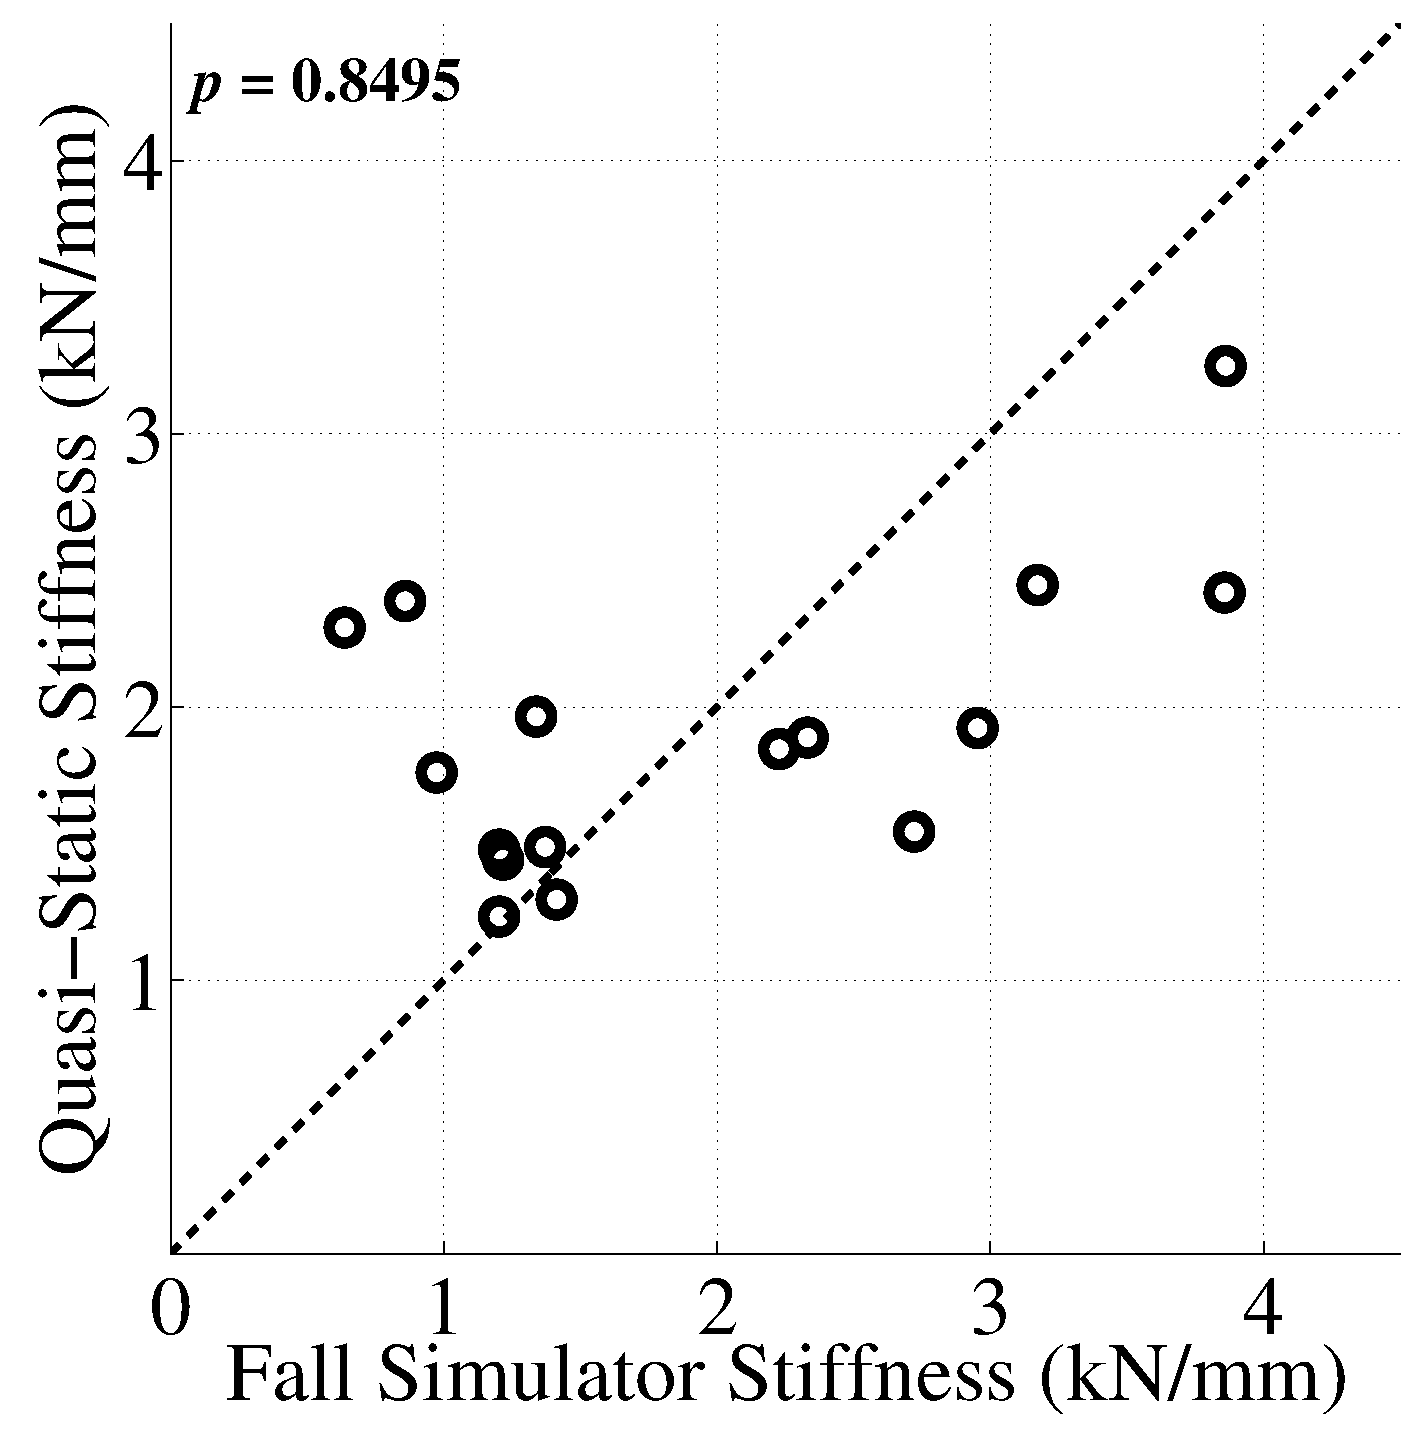
\includegraphics[width=\linewidth]{./appendixPlots/figures/StiffnessVsStiffness}
\caption[Quasi-static vs.\ fall simulator stiffness]{\textbf{Average stiffness in the quasi-static and fall simulator tests up to the maximum load applied in the quasi-static testing}. Graphic \copyright Seth Gilchrist, 2013.}
\label{fig:StiffnessVsStiffness}
\end{figure}
\clearpage

\begin{figure}[h]
\centering
\includegraphics[width=\linewidth]{./appendixPlots/figures/EnergyVsEnergy}
\caption[Quasi-static vs.\ fall simulator energy]{\textbf{Energy absorbed by the fall simulator and the quasi-static tests upto the maximum force applied in the quasi-static tests.} Graphic \copyright Seth Gilchrist, 2013.}
\label{fig:EnergyVsEnergy}
\end{figure}
\clearpage

\begin{figure}
\centering
\includegraphics[width=\linewidth]{./appendixPlots/figures/DXA_DeltStrain}
\caption[\acs*{abmd} grouped by strain]{\textbf{\ac{abmd} of fall specimens grouped by their relative strains up to the maximum force applied in the QS condition, in the FS and QS conditions.} Graphic \copyright Seth Gilchrist, 2013.}
\label{fig:DXA_DeltStrain}
\end{figure}
\clearpage

\begin{figure}
\centering
\includegraphics[width=\linewidth]{./appendixPlots/figures/DXA_DeltaEng}
\caption[\acs*{abmd} grouped by energy]{\textbf{\ac{abmd} of fall specimens grouped by the relative energy up to the maximum force applied in the QS condition, in the FS and QS conditions.} Graphic \copyright Seth Gilchrist, 2013.}
\label{fig:DXA_DeltaEng}
\end{figure}
\clearpage

\section{Constant rate \acs*{vs} fall simulator}
\label{sec:additional_CR_FS_ratesIdeal}

\begin{figure}[h]
\centering
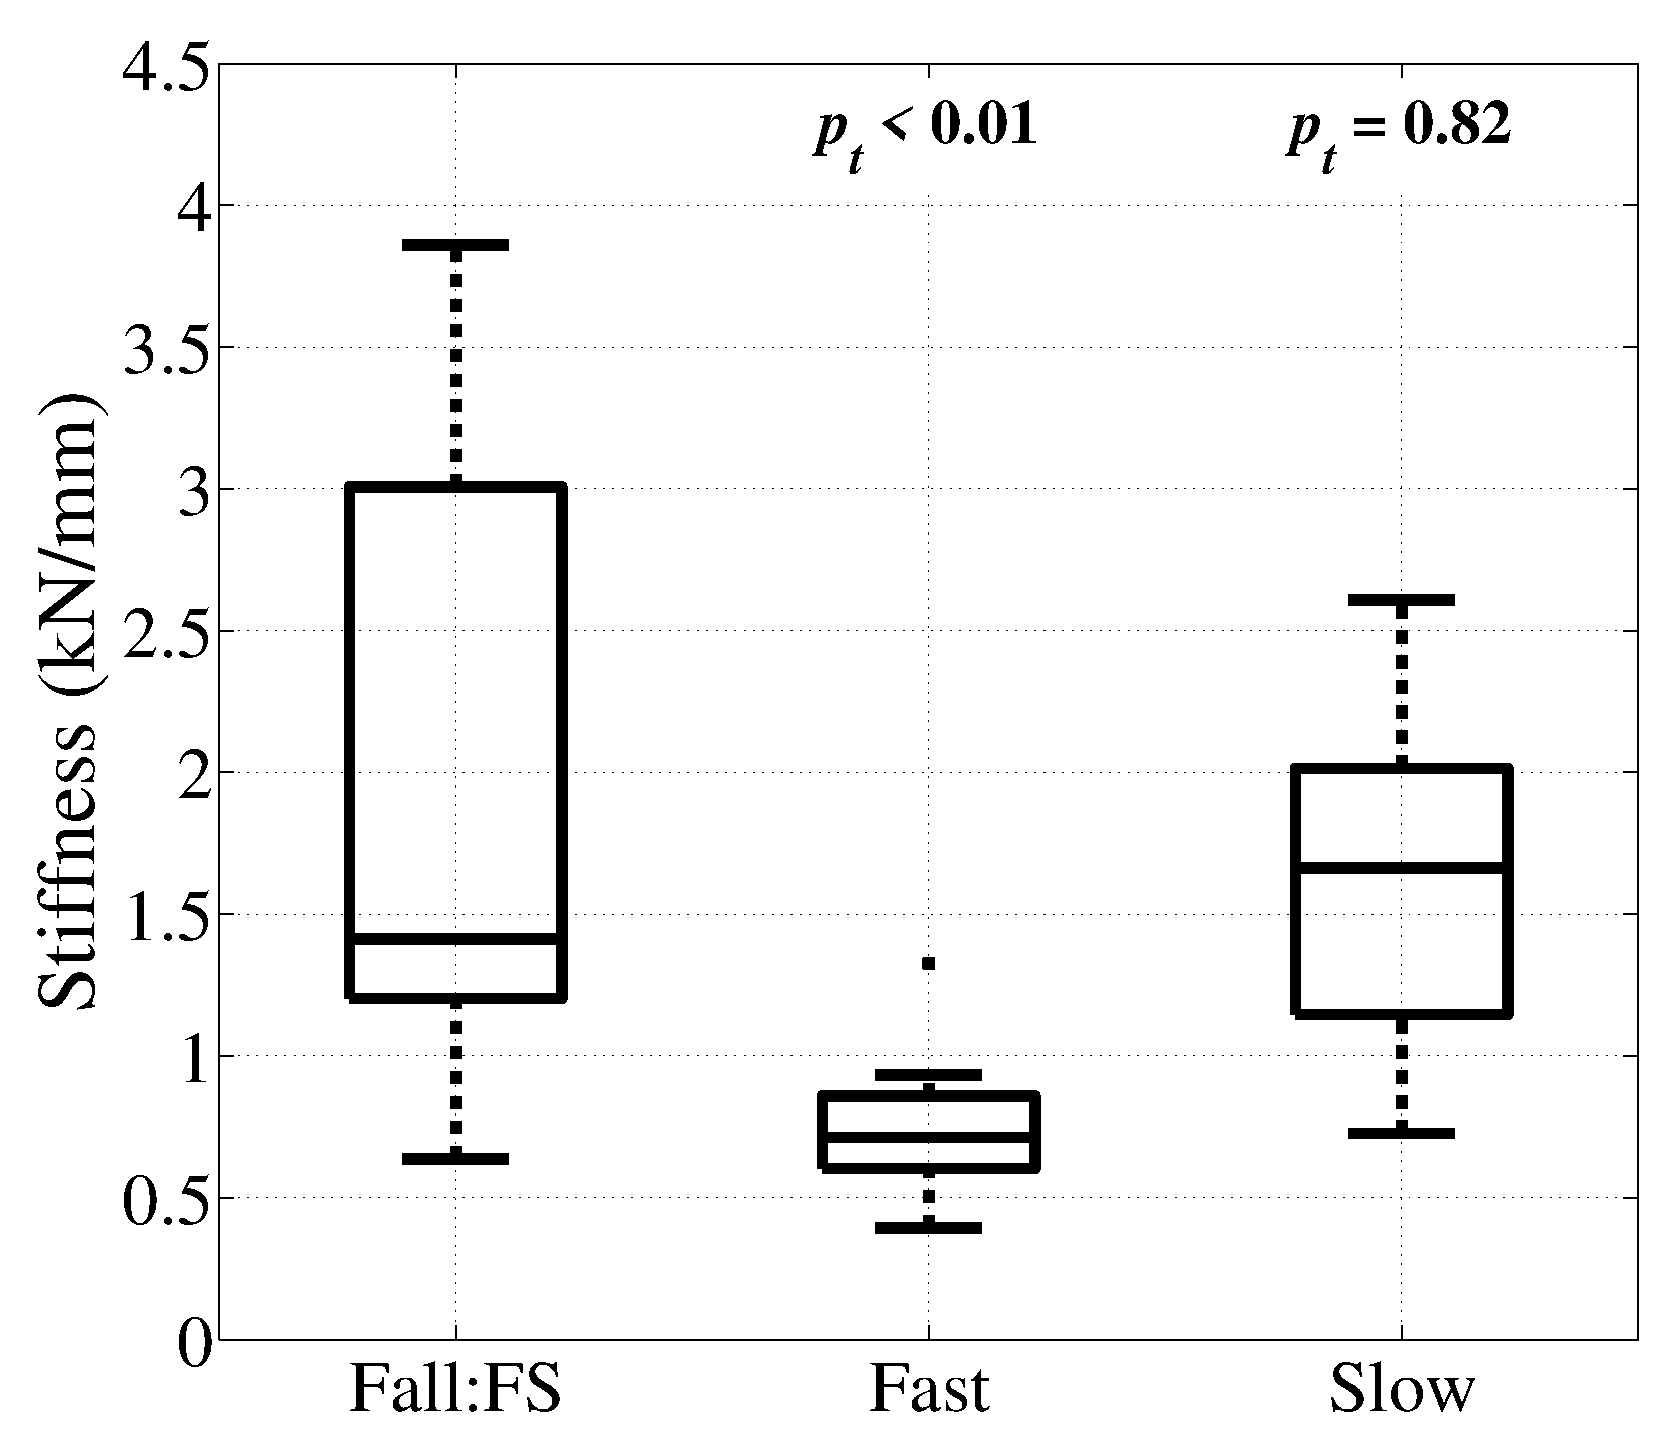
\includegraphics[width=\linewidth]{./appendixPlots/figures/StiffnessAll}
\caption[Stiffness of groups in failure tests]{\textbf{Stiffness of the fall:FS, fast and slow groups in the failure tests.} Graphic \copyright Seth Gilchrist, 2013.}
\label{fig:StiffnessAll}
\end{figure}
\clearpage

\begin{figure}[h]
\centering
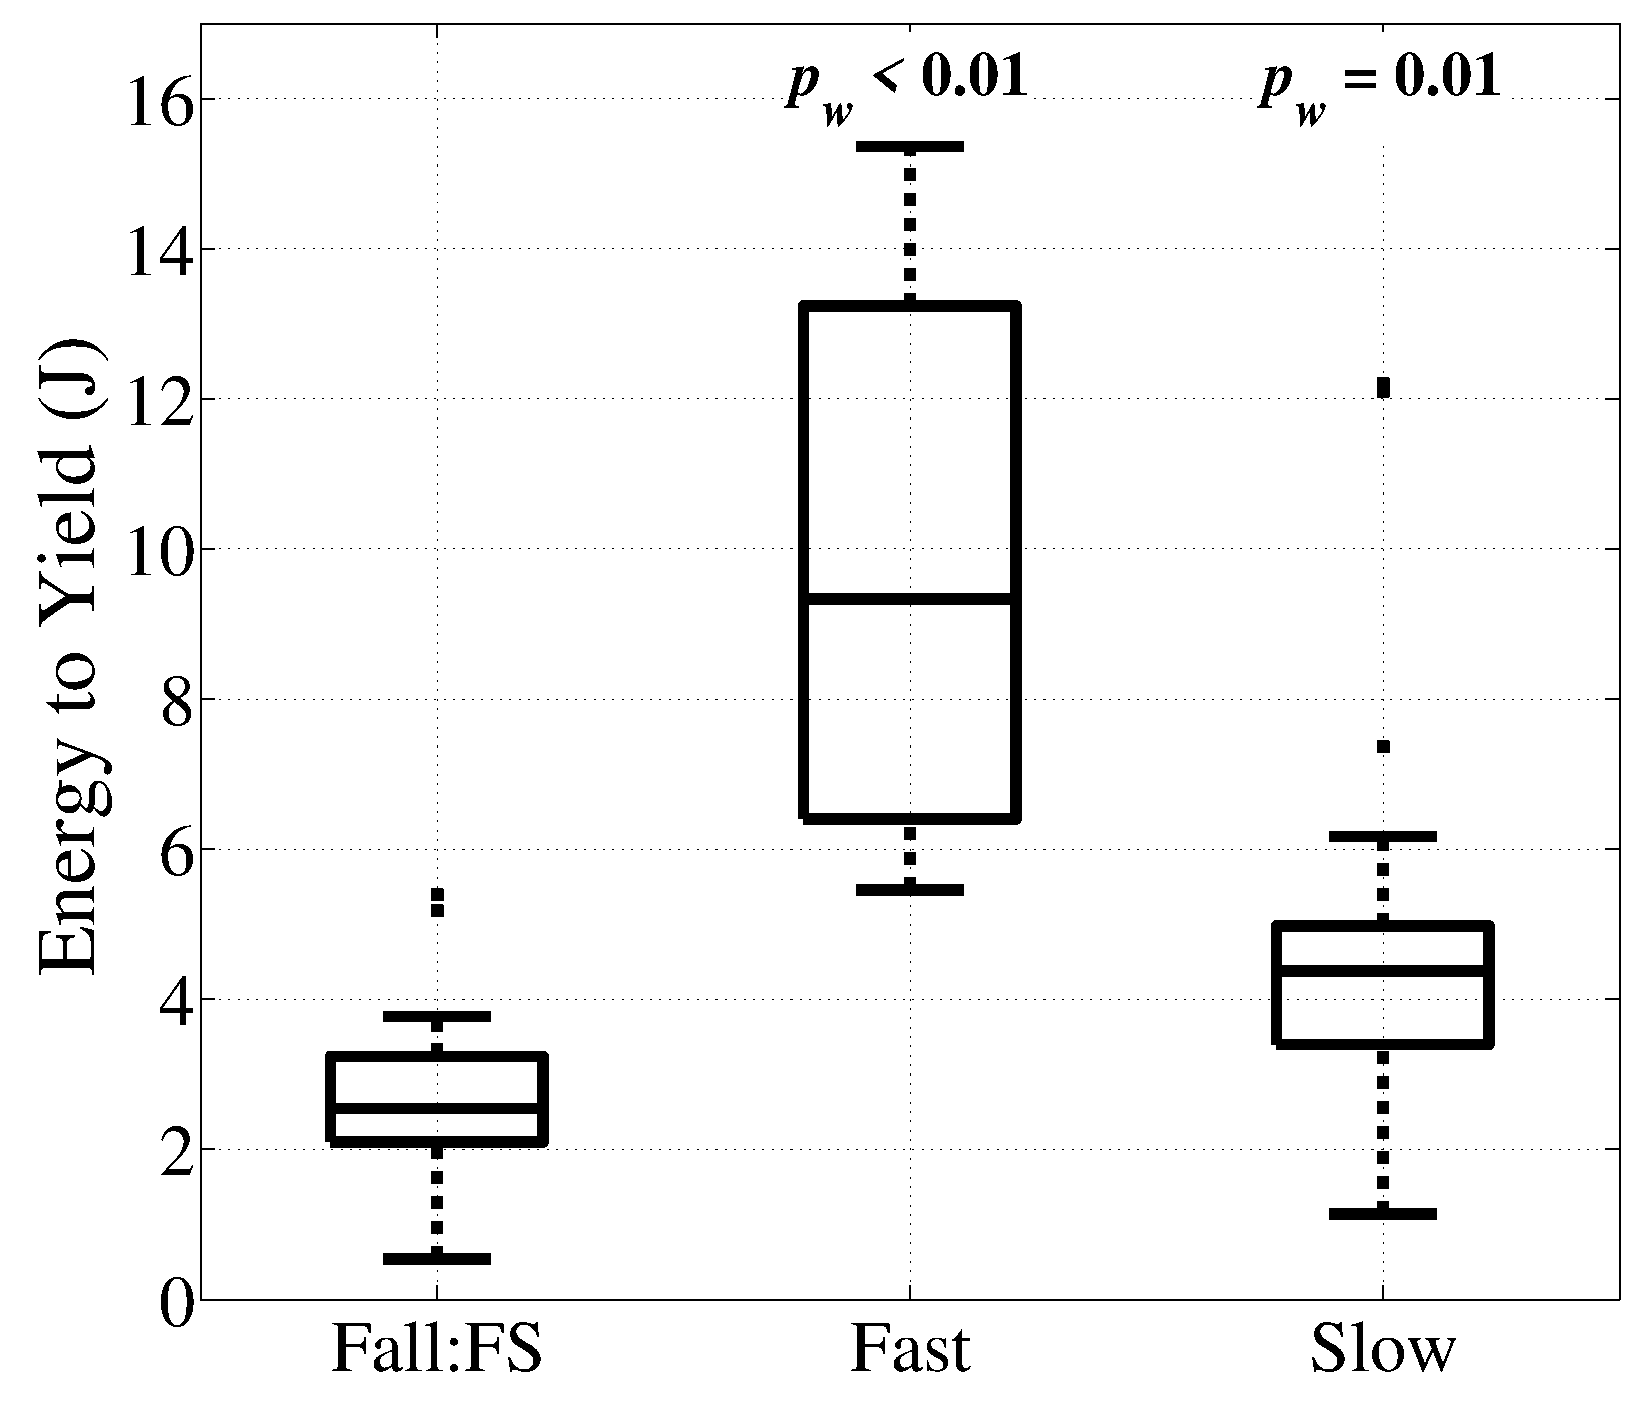
\includegraphics[width=\linewidth]{./appendixPlots/figures/EnergyAll}
\caption[Energy to yield in failure tests]{\textbf{Energy to yield in the fall:FS, fast and slow groups in the failure tests.} Graphic \copyright Seth Gilchrist, 2013.}
\label{fig:EnergyAll}
\end{figure}
\clearpage

\begin{figure}[h]
\centering
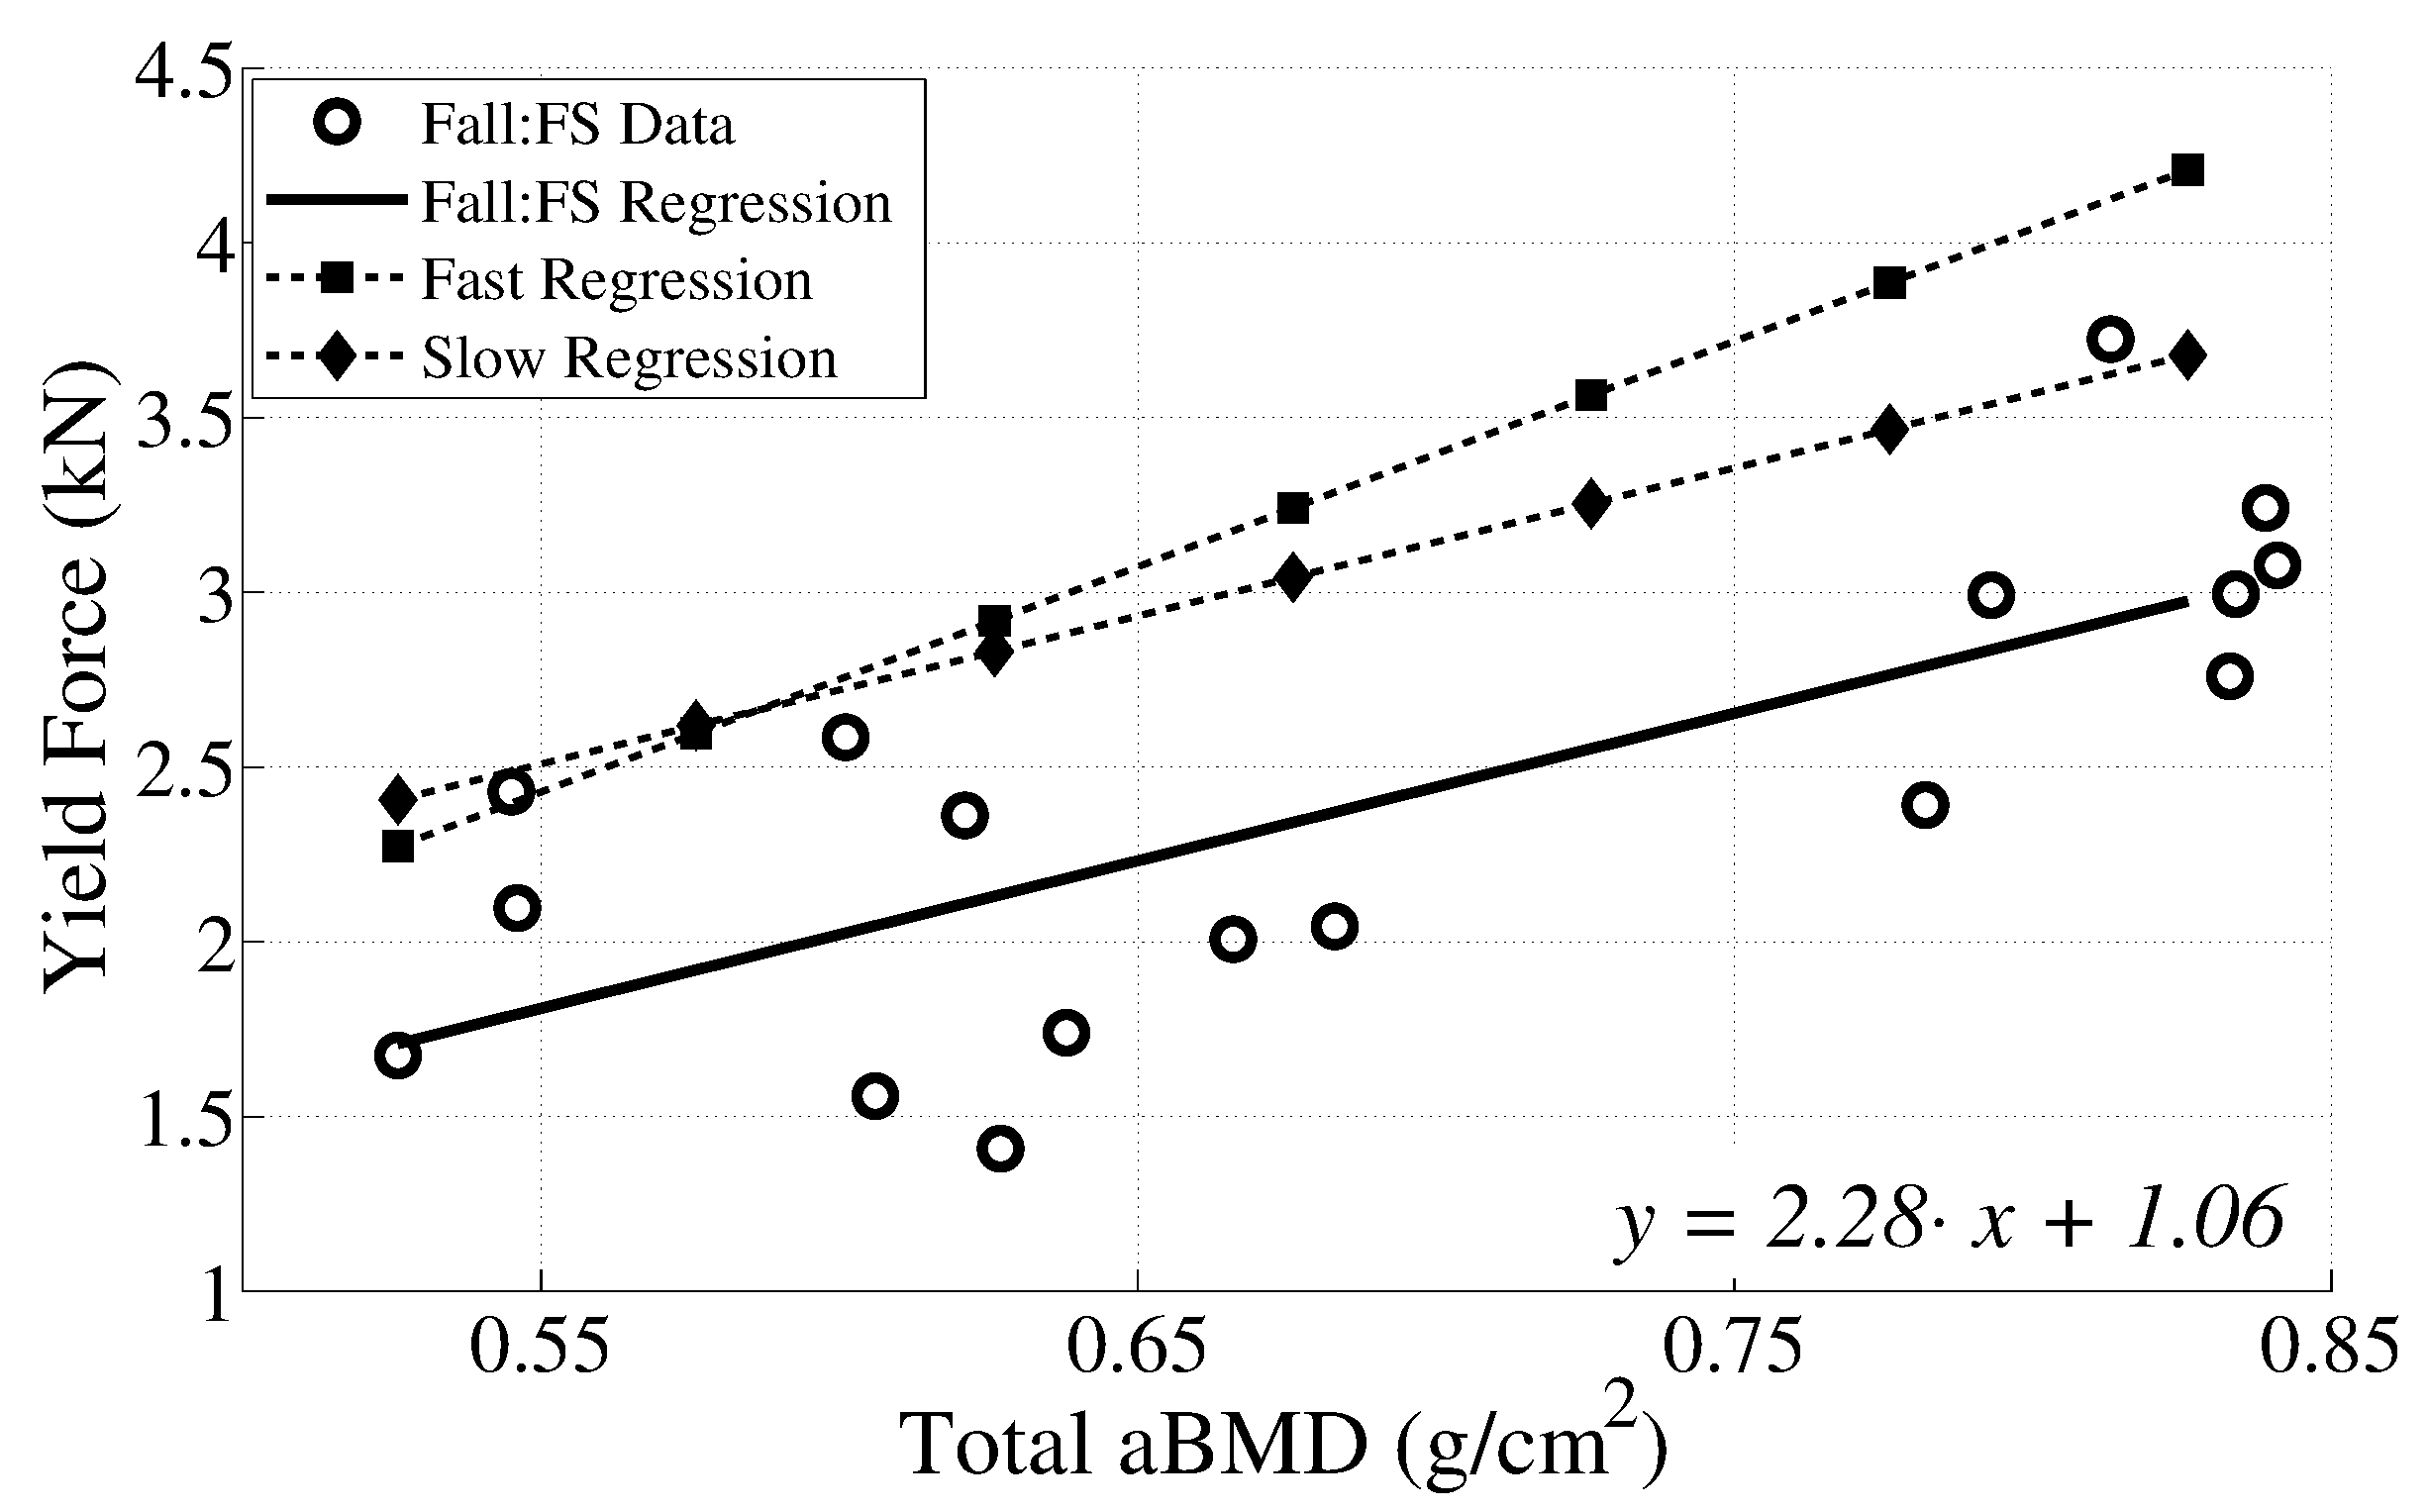
\includegraphics[width=\linewidth]{./appendixPlots/figures/MaxForceVsDXA}
\caption[Yield force vs.\ total \ac{abmd} in failure tests]{\textbf{The yield force as a function of total \ac{abmd} in the failure tests. The equation is the regression for the current results.} Graphic \copyright Seth Gilchrist, 2013.}
\label{fig:MaxForceVsDXA}
\end{figure}
\clearpage


